\documentclass{article}
\usepackage[margin=2.5cm]{geometry}
\usepackage{kotex}
\usepackage{titlesec}
\usepackage{amsmath}
\usepackage{listings}
\usepackage{amssymb}
\usepackage[bottom]{footmisc}
\usepackage{hyperref} % For clickable referneces and a structure view of pdf.
\usepackage{graphicx}
\graphicspath{{figures/}}

\usepackage{natbib}
\bibliographystyle{plainnat}
\setcitestyle{authoryear,open={(},close={)}}

\title{Linear Algebra Crash Course}
\author{Sungjun Eom}
\date{\today}

\titleformat{\section}[hang]
{\normalfont\bfseries\LARGE}
{\thesection.}{0.5em}{}

\titleformat{\subsection}[hang]
{\normalfont\bfseries\Large}
{\thesubsection}{0.4em}{}

\titleformat{\subsubsection}[hang]
{\normalfont\bfseries\large}
{\thesubsubsection}{0.3em}{}

\begin{document}

\maketitle

\tableofcontents

\newpage

\section{Vector Spaces and Subspaces}

\section{Linear Independence}
If there are only zero \(\alpha_i\) for all i which satisfy the equation below, we say a set of vectors \(\{x_1, \dots, x_n\}\) is linearly independent.
\begin{align}
\alpha_1 x_1+\alpha_2 x_2 + \dots + \alpha_n x_n = 0
\end{align}


\section{Basis, Representation and Orthonormalization}


\subsection{Basis}
Basis is a set of linearly independent vectors \(\{x_1, \dots, x_n\}\) which is used to form an n-dimensional space. \(\iff\) Basis \(\{x_1, \dots, x_n\}\) spans n-dimensional space.

\subsection{Representation}
In this subsection, we restrict vectors to arrays. Representation of vectors and representation of matrices are introduced differently in this article.


\subsubsection{Vector}
\(x\) is a vector whose basis is \(I\). \(Q\) is a new basis on which we want to represent the vector. \(\bar{x}\) is a representation for the vector \(x\) with respect to the basis \(Q\).\footnote{Actually we cannot say Q is a basis. Q is just a matrix made up of vectors of the basis.}
\begin{align}
x = Q\bar{x}
\end{align}
We assume the basis \(Q\) is formed by stacking linearly independent column vectors \(q_1, q_2,\dots,q_n\).
\begin{align*}
Q := \left[ \begin{matrix} q_1 & q_2 & \dots & q_n \end{matrix}\right]
\end{align*}


\subsubsection{Matrix}
A representation of matrix \(A\) is \(\bar{A}\). \(\bar{A}_i\) means the \(i^{th}\) column of the basis \(Q\).
\begin{align} \label{eq:1}
Aq_i=Q\bar{A}_i
\end{align}
Why does the representation of a matrix look like this? What we really want to do is actually this: to represent \(y=Ax\) in another form \(\bar{y}=\bar{A}\bar{x}\). So we should start from the equation \(y=Ax\).
\begin{align*}
y&=Ax \\
Q\bar{y}&=AQ\bar{x} \\
\end{align*}
Suppose \(Q\) is an \(n \times n\) matrix. The matrix \(Q\) consists of vectors from the basis so the column vectors of the matrix are linearly independent. Then the matrix \(Q\) is invertible.
\begin{align*}
\bar{y}&=Q^{-1}AQ\bar{x} \\
\bar{y}&=\bar{A}\bar{x}
\end{align*}
We get the equation:
\begin{align} \label{eq:similarity_transform}
\bar{A} &= Q^{-1}AQ
\end{align}
Next we go forward to get the equation \ref{eq:1}.
\begin{align*}
AQ&=Q\bar{A}\\
A\left[\begin{matrix} q_1 & \dots & q_n\end{matrix} \right]
&= Q\left[\begin{matrix} \bar{A}_1 & \dots & \bar{A}_n\end{matrix} \right] \\
\left[\begin{matrix} Aq_1 & \dots & Aq_n\end{matrix} \right]
&= \left[\begin{matrix} Q\bar{A}_1 & \dots & Q\bar{A}_n\end{matrix} \right]
\end{align*}
If we choose \(i^{th}\) column then we get the equation \ref{eq:1} \(Aq_i=Q\bar{A}_i\).
\citep{Chen_2014}

\subsection{Orthonormalization}
\subsubsection{Orthonormal}
Two vectors \(v_1\) and \(v_2\) are \textbf{orthogonal} if and only if
\begin{align*}
v_1^Tv_2=0
\end{align*}
If all orthogonal vectors in a set have magnitude one then we say them \textbf{orthonormal}.
\begin{align*}
||v_i|| = 1 \quad or \quad v_i^Tv_i=1
\end{align*}

\subsubsection{Gram-Schmidt process}
Suppose we have vectors \(e_1, e_2, \dots ,e_n\) which we want to orthonormalize. The following steps are called Gram-Schmidt processs and are used to make orthonormal vectors \(q_1, q_2, \dots, q_n\).
\begin{align*}
v_1 := e_1 &\qquad \qquad q_1 := \frac{v_1}{||v_1||}\\
v_2 := e_2 - q_1^Te_2 &\qquad \qquad  q_2 := \frac{v_2}{||v_2||}\\
v_3 := e_3 - q_1^Te_3 - q_2^Te_3 &\qquad \qquad  q_2 := \frac{v_3}{||v_3||}\\
&\vdots\\
v_n := e_n - \sum_{i=1}^{n-1}q_i^Te_n &\qquad \qquad q_n := \frac{v_n}{||v_n||}
\end{align*}
This process incremently removes the effect of former vectors from the current vector and normalizes the current vector.
\section{Linear Algebraic Equation}
A linear algebraic equation is:
\begin{align} \label{eq: LAE}
\mathbf{y}_{n\times 1}=\mathbf{A}_{n \times m}\mathbf{x}_{m \times 1}
\end{align}

\subsection{Projection}
Let \(\{z_1, \dots, z_n \}\) be an orthonormal basis for \(\mathbb{R}^n\), \(\{z_1, \dots, z_r \}\) be basis for \(V\), and \(\{z_{r+1}, \dots, z_n \}\) be basis for \(V^\perp\). Next, we form matrices:
\begin{align*}
Z= \left[ \begin{matrix}z_1 & \dots & z_n\end{matrix} \right]_{n\times n} ,
\quad Z_1 = \left[ \begin{matrix}z_1 & \dots & z_r\end{matrix} \right]_{n\times r},
\quad Z_2 = \left[ \begin{matrix}z_{r+1} & \dots & z_n\end{matrix} \right]_{n\times n-r}
\end{align*}
\(C(Z)\) means a space spanned by column vectors of Z. Then the equations below hold.
\begin{align*}
\mathbb{R}^n=C(Z)=span(\{z_1,\dots,z_n\}), \quad
V = C(Z_1)=span(\{z_1,\dots,z_r\}), \quad
V^\perp = C(Z_2)=span(\{z_{r+1}, \dots, z_n\})
\end{align*}
Just to be clear, we write relations between them.
\begin{align*}
V \subset \mathbb{R}^n, \quad V^\perp \subset \mathbb{R}^n, \quad V \perp V^\perp
\end{align*}
\paragraph{Definition of projection:} We say a linear mapping \(\pi_V: \mathbb{R}^n \rightarrow V\) is a projection onto \(V\) when the equation below holds.
\begin{align*}
\forall \mathbf{v}\in V, \quad \forall \mathbf{x}\in \mathbb{R}^n, \quad <\mathbf{v}, \pi_V(\mathbf{x})-\mathbf{x}>=0
\end{align*}
\paragraph{Definition of projection matrix:} \(P\) is a projection matrix when the following equation holds. 
\begin{align*}
\pi_V(\mathbf{x})=P\mathbf{x}
\end{align*}
\(Z_1Z_1^T\) is a projection matrix onto \(V\). Likewise \(Z_2Z_2^T\) is a projection matrix onto \(V^\perp\). We verify this:\\
For \(\forall \mathbf{x} = Z\alpha \in \mathbb{R}^n\),
\begin{align*}
Z_1Z_1^T\mathbf{x}&=Z_1Z_1^TZ\alpha\\
&=Z_1Z_1^T\left[\begin{matrix}Z_1 & Z_2\end{matrix}\right]\alpha\\
&=Z_1Z_1^T\left(Z_1\alpha_1+ Z_2\alpha_2\right)\\
&=Z_1Z_1^TZ_1\alpha_1 + Z_1Z_1^TZ_2\alpha_2\\
&=Z_1\alpha_1
\end{align*}
We used the fact that \(Z_1^TZ_1=I\). Also, notice that \(I-Z_1Z_1^T\) is a projection matrix onto \(V^\perp\) and \(I-Z_2Z_2^T\) is a projection matrix onto \(V\).

In the paragraph above, we only consider the case of orthogonal \(Z\)s. The next question which arises will be how we form a projection matrix when the matrices don't have orthonormal column vectors. Although a matrix doesn't have orhtonormal columns, we can make them be orthonormal. For example, Gram-Schmidt process. So there is always a matrix \(A_{r\times r}\) which converts vectors of a matrix \(X_{n \times r}\) to be orthonormal.
\begin{align*}
Z_1 = XA
\end{align*}
Use what we already know:
\begin{align*}
Z_1 Z_1^T&=XA A^T X^T\\
\&\\
I_r = Z_1^TZ_1 &= A^TX^TXA\\
\iff (A^T)^{-1}A^{-1}&=X^TX\\
AA^T&=(X^TX)^{-1}
\end{align*}
Finally, we get the equation below.
\begin{align*}
\therefore Z_1Z_1^T&=X(X^TX)^{-1}X^T
\end{align*}
This is a projection matix onto \(V\). Likewise, \(I-X(X^TX)^{-1}X^T\) is a projection matrix onto \(V^\perp\).\\
We conclude that the projection onto V is:
\begin{align*}
\pi_V(x)=X(X^TX)^{-1}X^Tx
\end{align*}
And its projection matrix is:
\begin{align*}
P_\pi=X(X^TX)^{-1}X^T
\end{align*}
One thing we should keep in mind is that a projection matrix is an idempotent matrix. Refer to \ref{subsection: idempotent}.

\subsection{Least Square Method}
Consider a linear model \(y=X\beta +\epsilon\).
We want to minimize the square sum of errors \(\epsilon^T\epsilon=\epsilon_1^2+\dots+\epsilon_n^2\).
\begin{align*}
e^Te &= (y-X\beta)^T(y-X\beta) \\
&= <y-X\beta, y-X\beta> \\
&= <y-X\beta,y-X\beta> \\
&= <y-\pi_V(y)+\pi_V(y)-X\beta,y-\pi_V(y)+\pi_V(y)-X\beta>\\
\begin{split}
&= <y-\pi_V(y),y-\pi_V(y)> + 2<y-\pi_V(y),\pi_V(y)-X\beta>\\
&\qquad \qquad+<\pi_V(y)-X\beta,\pi_V(y)-X\beta>
\end{split}
\end{align*}
Because \(y-\pi_V(y)\) is in \(V^\perp\) and \(\pi_V(y)-X\beta\) is in \(V\), \(<y-\pi_V(y),\pi_V(y)-X\beta>\) is zero.
\begin{align*}
e^Te &=\quad<y-\pi_V(y),y-\pi_V(y)>+<\pi_V(y)-X\beta,\pi_V(y)-X\beta>\\
&\geq\quad <\pi_V(y)-X\beta,\pi_V(y)-X\beta>
\end{align*}
The square sum of errors is minimized when:
\begin{align*}
\pi_V(y)&=X\beta=X(X^TX)^{-1}X^Ty\\
\beta &= (X^TX)^{-1}X^Ty
\end{align*}
\begin{figure}[hb]
\centering
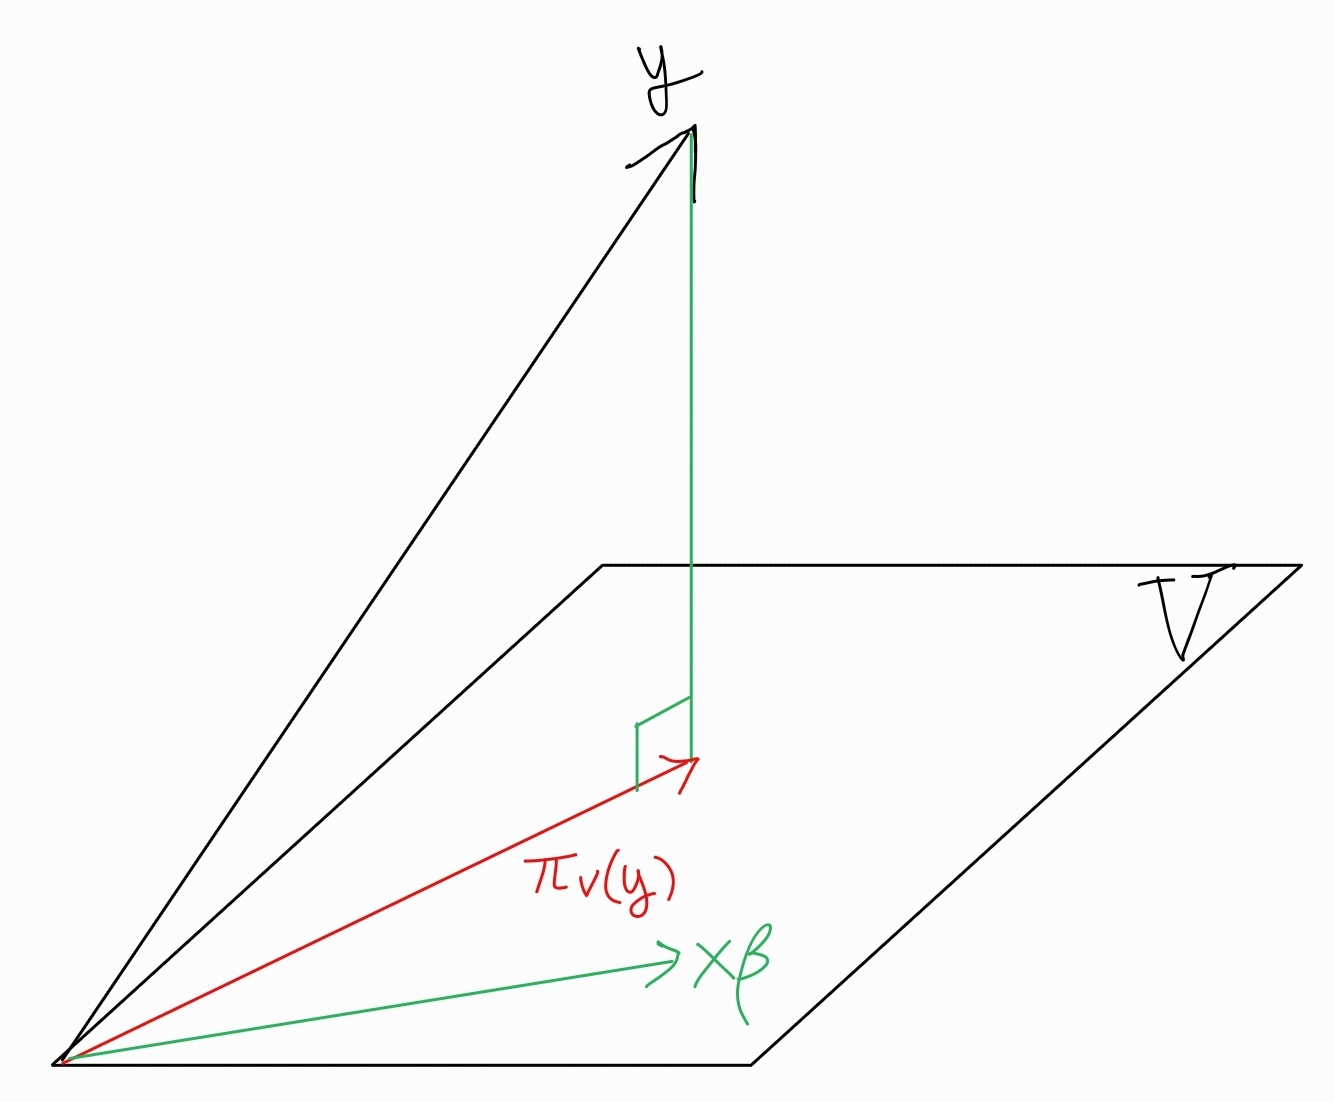
\includegraphics[scale=0.2]{fig_1.jpg}
\caption{Visualization of Least Square Method}
\end{figure}

\subsection{Generalized Inverses}
\paragraph{Penrose Conditions:} There exists a unique solution \(X\) for any \(A\).
\begin{align} \label{eq: generalized inverse}
AXA &= A \\
XAX &= X \\
(AX)^* &= AX \\
(XA)^* &= XA
\end{align}
\(X\) is a Moore-Penrose inverse of \(A\) \citep{Penrose_1955}. The matrix \(X\) satisfying the conditions above is unique. The equation \ref{eq: generalized inverse} alone is not unique in general but it is sufficient for most cases. We say the matrix \(X\) satisfying the equation \ref{eq: generalized inverse} is a generalized inverse of \(A\) \citep{Searle_Khuri_2017}.


\section{Similarity Transformation}


\section{Diagonal Form and Jordan Form}

\subsection{Eigenvalues and Eigenvectors}

\subsection{Eigendecomposition}

\subsection{Multiplicities}

\subsubsection{Algebraic Multiplicities}

\subsubsection{Geometric Multiplicities}

\subsection{Generalized Eigenvectors}

\subsection{Jordan Form}

\section{Functions of a Square Matrix}

\subsection{Polynomials}

\subsection{Cayley-Hamilton Theorem}

\subsection{Exponentials}

\section{Sylvester's Equation}

\subsection{Solution with a Vec Operator}

\subsection{Eigenvalues}

\section{Some Useful Formulas}

\subsection{Ranks}

\subsection{Diagonal Expansion}

\subsection{Determinants}

\section{Special Matrices}

\subsection{Symmetric Matrices}

\subsection{Idempotent Matrices} \label{subsection: idempotent}

\section{Quadratic Forms and Positive Definiteness}

\subsection{Quadratic Forms}

\subsection{Positive Definiteness}

\section{Singular Value Decomposition}

\subsection{Singular Value}

\subsection{Singular Value Decomposition}

\section{Norms of Matrices}

\section{Matrix Calculus}

\newpage

\bibliography{refs}

\end{document}
